\documentclass{standalone}
\usepackage{tikz,trees}
\begin{document}
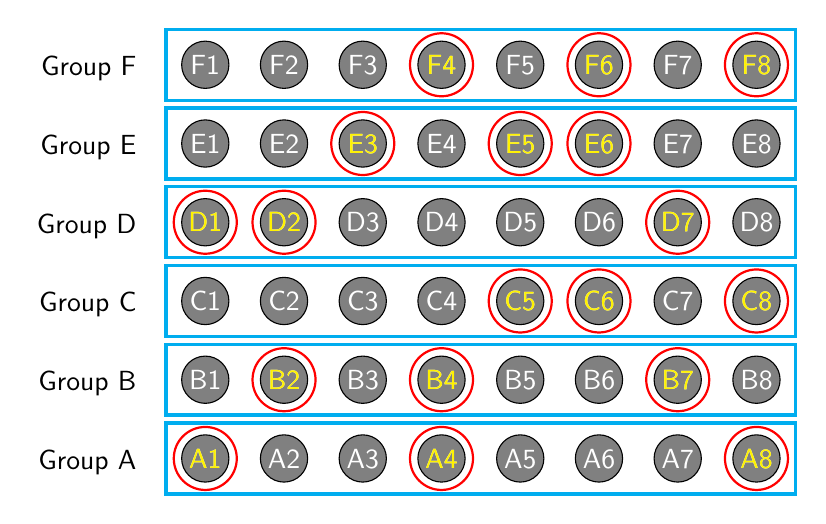
\begin{tikzpicture}[font=\sffamily]
  \edef\gnames{{"A","B","C","D","E","F"}};

  % Draw group backgrounds and labels (once per group)
  \foreach \grp in {1,2,...,6} {
      \pgfmathsetmacro\gname{\gnames[\grp-1]};
      \draw[cyan,very thick] (-0.5,{\grp-0.45}) rectangle (7.5,{\grp+0.45});
      \node[left] at (-0.75,{\grp-0.05}) {Group \gname};
  }

  % Draw all circles
  \foreach \grp in {1,2,...,6} {
      \pgfmathsetmacro\gname{\gnames[\grp-1]};
      \foreach \num in {1,2,...,8} {
          \draw[fill=gray] ({\num-1},\grp) circle (0.3) node[white] (\num) {\gname\num};
      }
  }

  % Define sample data and draw red circles
  \edef\sample{{
      {1,4,8},
      {2,4,7},
      {5,6,8},
      {1,2,7},
      {3,5,6},
      {4,6,8}
  }}
  \foreach \grp in {1,2,...,6} {
      \pgfmathsetmacro\gname{\gnames[\grp-1]};
      \foreach \i in {1,2,3} {
          \pgfmathsetmacro\num{\sample[\grp-1][\i-1]};
          \draw[draw=red,thick] ({\num-1},\grp) circle (0.4) node[yellow] {\gname\num};
      }
  }
\end{tikzpicture}
\end{document}